\documentclass{beamer}
\usetheme{Boadilla} 
\setbeamercovered{invisible}
\setbeamertemplate{navigation symbols}{} 
%\useoutertheme{infolines} 

\usepackage[utf8]{inputenc}
\usepackage{graphicx}

\setbeamertemplate{frametitle continuation}{} 
\usepackage{subfigure}
\usepackage{caption}
\usepackage{bm}
\usepackage{epsfig}

\usepackage{amsmath}
\usepackage{xcolor,colortbl}

\usepackage{multicol}
\usepackage{wasysym}

\usepackage{hyperref}
\usepackage{float}

\usepackage{array}
\newcolumntype{L}[1]{>{\raggedright\let\newline\\\arraybackslash\hspace{0pt}}m{#1}}
\newcolumntype{C}[1]{>{\centering\let\newline\\\arraybackslash\hspace{0pt}}m{#1}}
\newcolumntype{R}[1]{>{\raggedleft\let\newline\\\arraybackslash\hspace{0pt}}m{#1}}

\usepackage[T1]{fontenc}
\usepackage{tikz}
\usetikzlibrary{shadows}

\newcommand*\keystroke[1]{%
  \tikz[baseline=(key.base)]
    \node[%
      draw,
      fill=white,
      drop shadow={shadow xshift=0.25ex,shadow yshift=-0.25ex,fill=black,opacity=0.75},
      rectangle,
      rounded corners=2pt,
      inner sep=1pt,
      line width=0.5pt,
      font=\scriptsize\sffamily
    ](key) {#1\strut}
  ;
}

% deal with spaces in absolute paths

\usepackage[space]{grffile}
\graphicspath{{C:/Users/Yered/Dropbox/Harvard/Winter 2014/CdeC/Slides/Introduction/figures/}}

\usepackage[scaled]{helvet}
\usepackage[round]{natbib}


\begin{document}
\title[Datos de Expresi\'{o}n Gen\'{e}tica]{Explorando el Transcriptoma con Datos de Expresi\'{o}n Gen\'{e}tica\\
\vspace{0.5cm}
Datos de Expresi\'{o}n Gen\'{e}tica}
\author{Yered Pita-Ju\'{a}rez}
\institute[CdeC M\'{e}rida]{}
\date{6/1/2015}


\begin{frame}
\titlepage
\end{frame}

\begin{frame}[fragile]{ALL}
\begin{itemize}
\item 128 pacientes con leucemia linfoide aguda (acute lymphoid leukemia)
\item Afecta los los linfocitos en la médula ósea
\item Linfocitos: células del sistema inmune
\item Puede afectar
\begin{itemize}
	\item linfocitos B
	\item linfocitos T
\end{itemize}
\item Paquetes y datos
\begin{verbatim}
library("Biobase")
library("ALL")
library("genefilter")
data("ALL")
\end{verbatim}
\end{itemize}
\end{frame}

\begin{frame}[fragile]{ALL}
\begin{itemize}
\item 95 muestras con células B
\item 33 muestras con células T
\begin{verbatim}
ALL$BT 
\end{verbatim}
\item Seleccionar muestras con células B
\begin{verbatim}
bcell = grep("^B", as.character(ALL$BT))
\end{verbatim}
\item Dos tipos de muestras en células B: mutación BCR/ABL
\item Translocación: segmento del cromosoma 22 intercambiado con un segmento del cromosoma 9
\begin{verbatim}
types = c("NEG", "BCR/ABL")
moltyp = which(as.character(ALL$mol.biol) %in% types)
ALL_bcrneg = ALL[, intersect(bcell, moltyp)]
ALL_bcrneg$mol.biol = factor(ALL_bcrneg$mol.biol)
\end{verbatim}
\end{itemize}
\textbf{¿Qué genes están siendo expresados de manera diferente entre los tipos de leucemia de las células B?}
\end{frame}

\begin{frame}[fragile]{Filtrado}
\begin{itemize}
\item Buena parte de las sondas en el microarreglo no es muy informativa
\begin{itemize}
	\item el gen no está expresado
	\item la sonda no lo pudo detectar
\end{itemize}
\item Pre seleccionar genes basados en la desviación estándar
\item Poca variabilidad: no es posible distinguir si los genes estan siendo expresados de manera diferente
\end{itemize}
\end{frame}


\begin{frame}[fragile]{Filtrado}
\begin{itemize}
\item \verb=shorth=: promedio del intervalo más pequeño que contiene la mitad de las observaciones
\begin{verbatim}
library("genefilter")
sds = rowSds(exprs(ALL_bcrneg))
sh = shorth(sds)
sh
\end{verbatim}
\item Seleccionar las sondas con niveles de expresión por arriba de sh
\begin{verbatim}
ALLsfilt = ALL_bcrneg[sds>=sh, ]
dim(exprs(ALLsfilt))
dim(exprs(ALL_bcrneg))
\end{verbatim}
%\item Gráfica
%\begin{verbatim}
%hist(sds, breaks=50, col="mistyrose",
%     xlab="desviación estándar")
%abline(v=sh, col="blue", lwd=3, lty=2)
%\end{verbatim}
\end{itemize}
\end{frame}

\begin{frame}[fragile]{Filtrado}
\begin{itemize}
%\item \verb=shorth=: promedio del intervalo más pequeño que contiene la mitad de las observaciones
%\begin{verbatim}
%library("genefilter")
%sds = rowSds(exprs(ALL_bcrneg))
%sh = shorth(sds)
%sh
%\end{verbatim}
%\item Seleccionar las sondas con niveles de expresión por arriba de sh
%\begin{verbatim}
%ALLsfilt = ALL_bcrneg[sds>=sh, ]
%dim(exprs(ALLsfilt))
%dim(exprs(ALL_bcrneg))
%\end{verbatim}
\item Gráfica
\begin{verbatim}
hist(sds, breaks=50, col="mistyrose",
     xlab="desviación estándar",main="")
abline(v=sh, col="blue", lwd=3, lty=2)
\end{verbatim}
\end{itemize}
\begin{figure}
\centering
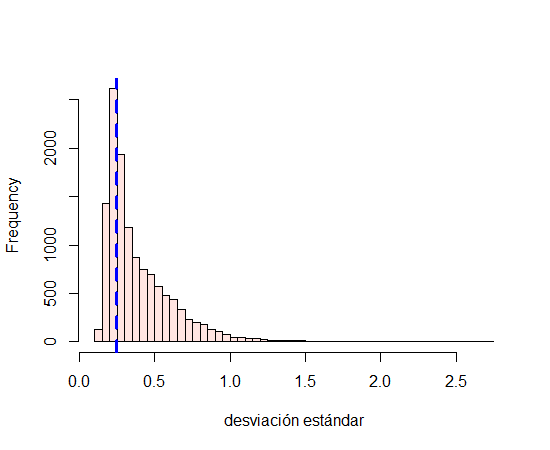
\includegraphics[scale=0.4]{all_sd_his.png}
\end{figure}
\end{frame}


\begin{frame}[fragile]{Prueba de t}
\begin{itemize}
\item Prueba de t para cada gen comparando los dos tipos de células B
\begin{verbatim}
table(ALLsfilt$mol.biol)
tt = rowttests(ALLsfilt, "mol.biol")
\end{verbatim}
\item Valores p
\begin{verbatim}
hist(tt$p.value, breaks=50, col="mistyrose",
     xlab="valor p",main="")
\end{verbatim}
\item Algunas sondas con valores p pequeños: genes diferencialmente expresados
\end{itemize}
\begin{figure}
\centering
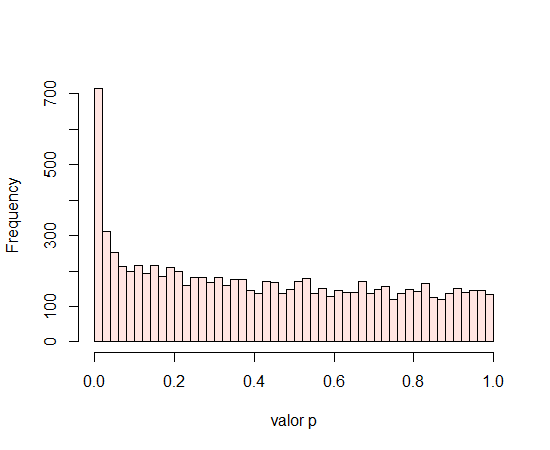
\includegraphics[scale=0.25]{all_hist_pval.png}
\end{figure}
\end{frame}

\begin{frame}[fragile]{Comparaciones Múltiples}
\begin{itemize}
\item Con un valor $\alpha$ de 0.05, vamos a rechazar la hipotesis nula en 441 casos (5\%) al azar
\item Ajustar el valor alpha
\begin{verbatim}
library("multtest")
mt = mt.rawp2adjp(tt$p.value, proc="BH")
\end{verbatim}
\item Los genes más significativos de acuerdo al valor p ajustado
\begin{verbatim}
g = featureNames(ALLsfilt)[mt$index[1:10]]
\end{verbatim}
\item Nombres
\begin{verbatim}
library("hgu95av2.db")
links(hgu95av2SYMBOL[g])
\end{verbatim}
\end{itemize}
\end{frame}



\begin{frame}[fragile]
\begin{block}{Ejercicio}
Trata de interpretar los genes que estan diferencialmente expresados.
\begin{verbatim}
> links(hgu95av2SYMBOL[g])
     probe_id  symbol
1     1635_at    ABL1
2   1636_g_at    ABL1
3     1674_at    YES1
4    32434_at  MARCKS
5    37015_at ALDH1A1
6    37027_at   AHNAK
7    39730_at    ABL1
8  39837_s_at  ZNF467
9    40202_at    KLF9
10   40504_at    PON2
\end{verbatim}
\end{block}

%\begin{figure}[H]
%\centering
%
\includegraphics[scale=0.15]{laptop.jpeg}
%\end{figure}
\end{frame}

\begin{frame}[fragile]{Comparaciones Múltiples}
\begin{itemize}
\item Gráfica
\begin{verbatim}
mb = ALLsfilt$mol.biol
y = exprs(ALLsfilt)[g[1],]
ord = order(mb)
plot(y[ord], pch=c(1,16)[mb[ord]],
     col=c("black", "red")[mb[ord]],
     main=hgu95av2SYMBOL[g[1]], ylab="Expresión",
     xlab="Muestras")
\end{verbatim}
\item Negro: Mutación
\item Rojo: Sin mutación 
\end{itemize}
\end{frame}

\begin{frame}[fragile]{Comparaciones Múltiples}
\begin{figure}[H]
\centering
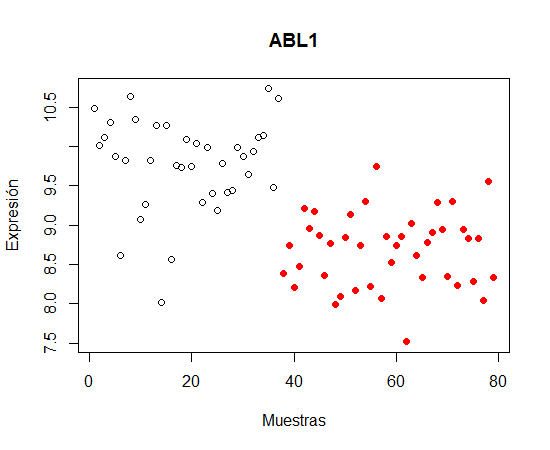
\includegraphics[scale=0.4]{ABL1_plot.png}
\end{figure}
\begin{itemize}
\item Abelson murine leukemia viral oncogene homolog 1 (ABL1) 
\item Proteína codificada por el gen ABL1
\item Gen localizado en el cromosoma 9
\end{itemize}
\end{frame}

\end{document}

\begin{frame}[fragile]{Comparaciones Múltiples}
\end{frame}

